\documentclass[a4paper]{article}
\usepackage[margin=10mm]{geometry}
\usepackage{xcolor}
\usepackage{tikz}
\usetikzlibrary{arrows.meta,calc}
\definecolor{lightbrown}{RGB}{222,184,135}
\definecolor{lightred}{RGB}{255,204,203}
\definecolor{palegreen}{RGB}{198,234,195}
\definecolor{paleblue}{RGB}{199,226,255}
\definecolor{palecoral}{RGB}{227,245,238}
\pagestyle{empty}
\begin{document}
\begin{center}
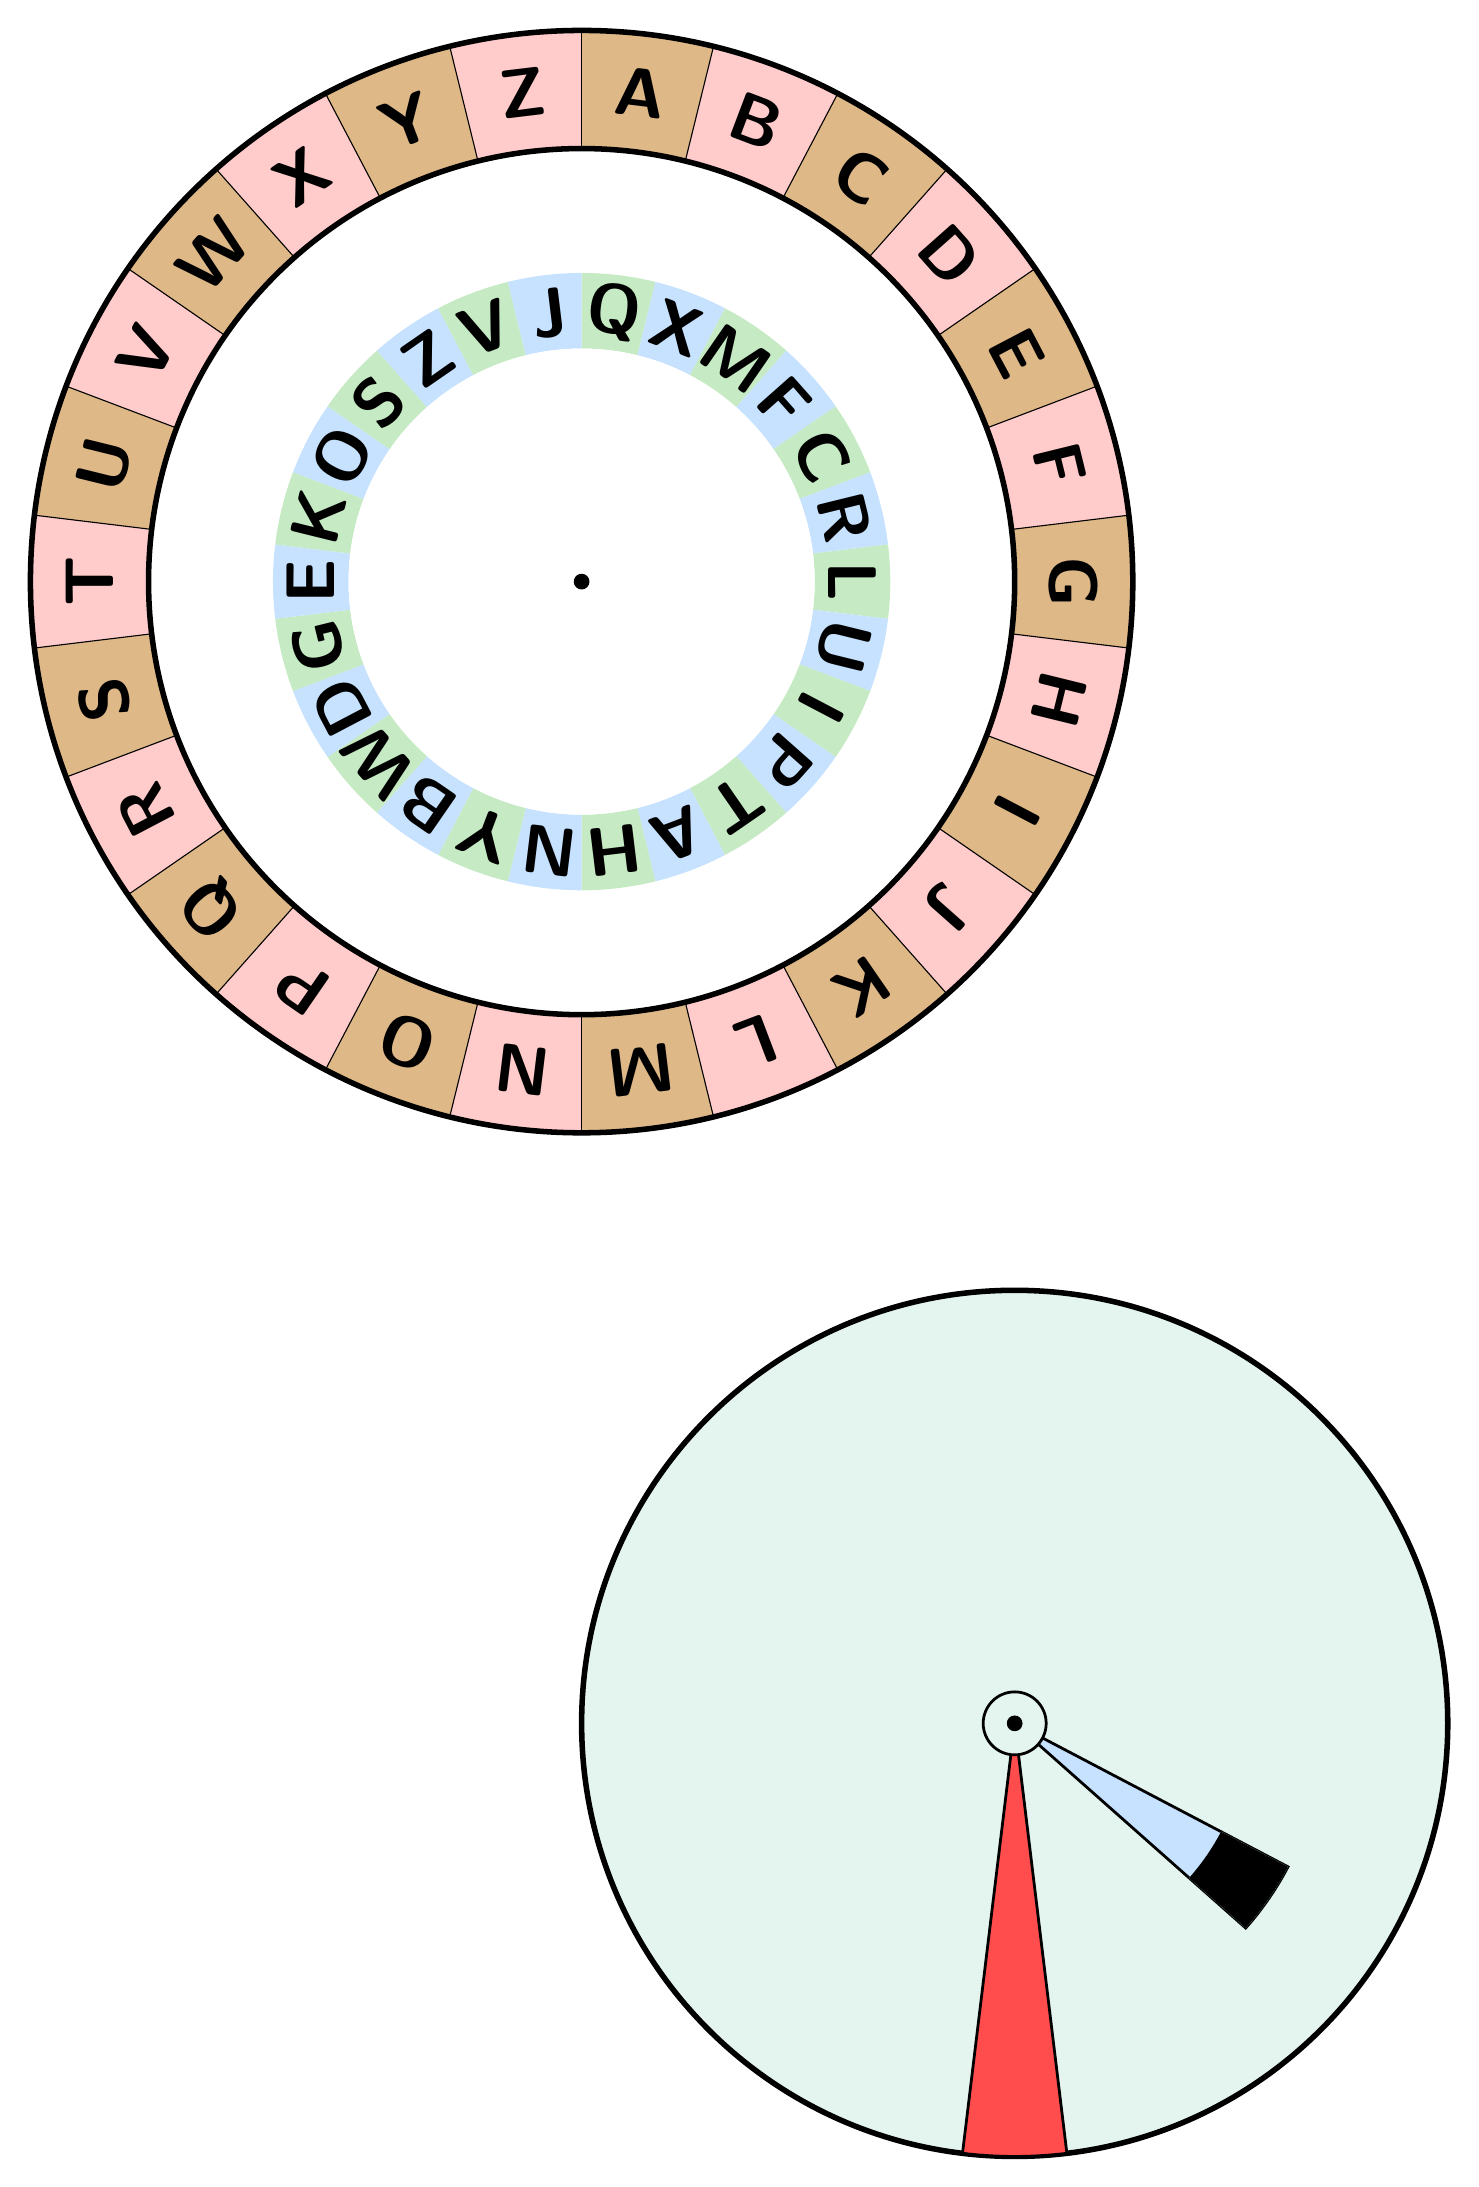
\begin{tikzpicture}[every node/.style={font=\sffamily\bfseries, inner sep=0pt, align=center}]
  % Outer static wheel
  \coordinate (O) at (-20mm,40mm);
  \def\outerRo{70mm}
  \def\outerRi{55mm}
  \def\outerLabelRo{62.5mm}
  \def\outerLabelRi{40mm}
  % decoded label radii moved 20% closer to centre
  \def\decodedLabelRo{39.2mm}
  \def\decodedLabelRi{29.6mm}
  \def\letterAngle{360/26}

  \foreach \i in {0,...,25} {
    \pgfmathsetmacro\angStart{90-\i*\letterAngle}
    \pgfmathsetmacro\angEnd{90-(\i+1)*\letterAngle}
    \ifodd\i
      \def\sectcolor{lightred}
    \else
      \def\sectcolor{lightbrown}
    \fi
    \fill[\sectcolor] ($(O)+(\angStart: \outerRi)$) -- ($(O)+(\angStart: \outerRo)$)
      arc (\angStart: \angEnd: \outerRo) -- ($(O)+(\angEnd: \outerRi)$)
      arc (\angEnd: \angStart: \outerRi) -- cycle;
  }

  \foreach \i in {0,...,25} {
    \pgfmathsetmacro\angStart{90-\i*\letterAngle}
    \pgfmathsetmacro\angEnd{90-(\i+1)*\letterAngle}
    \ifodd\i
      \def\sectcolor{paleblue}
    \else
      \def\sectcolor{palegreen}
    \fi
    \fill[\sectcolor] ($(O)+(\angStart: \decodedLabelRi)$) -- ($(O)+(\angStart: \decodedLabelRo)$)
      arc (\angStart: \angEnd: \decodedLabelRo) -- ($(O)+(\angEnd: \decodedLabelRi)$)
      arc (\angEnd: \angStart: \decodedLabelRi) -- cycle;
  }

  \fill[white] (O) circle (\decodedLabelRi);
  \draw[line width=2pt] (O) circle (\outerRo);
  \draw[line width=2pt] (O) circle (\outerRi);

  \foreach \i in {0,...,25} {
    \draw[line width=0.4pt] ($(O)+(90-\i*\letterAngle: \outerRi)$) -- ($(O)+(90-\i*\letterAngle: \outerRo)$);
  }

  \foreach \letter [count=\idx from 0] in {A,B,C,D,E,F,G,H,I,J,K,L,M,N,O,P,Q,R,S,T,U,V,W,X,Y,Z} {
    \pgfmathsetmacro\ang{90-(\idx+0.5)*\letterAngle}
    \node[font=\sffamily\bfseries\Huge, rotate=\ang-90] at ($(O)+(\ang: \outerLabelRo)$) {\letter};
  }

  \foreach \letter [count=\idx from 0] in {Q,X,M,F,C,R,L,U,I,P,T,A,H,N,Y,B,W,D,G,E,K,O,S,Z,V,J} {
    \pgfmathsetmacro\ang{90-(\idx+0.5)*\letterAngle}
    \node[font=\sffamily\bfseries\Huge, rotate=\ang-90] at ($(O)+(\ang: { (\decodedLabelRo + \decodedLabelRi)/2 })$) {\letter};
  }

  % Inner ring to cut out
  \coordinate (I) at (35mm,-105mm);
  \def\innerRo{\outerRi}
  \def\innerRi{25mm}
  \newlength{\letterheight}
  \settoheight{\letterheight}{\Huge A}
  \pgfmathsetlengthmacro\windowR{\letterheight/2}
  \def\windowAngle{95}
  \def\windowDist{\decodedLabelRo}
  \def\spindleR{4mm}
  \def\arrowAngle{72}

  \fill[palecoral] (I) circle (\innerRo);
  \draw[line width=2pt] (I) circle (\innerRo);
  % highlight one segment on Wheel 2 (angular width = one letter), centered at 0 degrees
  \pgfmathsetmacro\angCenter{-90}
  \pgfmathsetmacro\angStart{\angCenter + \letterAngle/2}
  \pgfmathsetmacro\angEnd{\angCenter - \letterAngle/2}
  \fill[red!70] (I) -- ($(I)+(\angStart: \innerRo)$) arc (\angStart: \angEnd: \innerRo) -- cycle;
  \draw[line width=1pt] (I) -- ($(I)+(\angStart: \innerRo)$) arc (\angStart: \angEnd: \innerRo) -- cycle;
  % second wedge rotated by 4 segments, stops at decodedLabelRo
  \pgfmathsetmacro\angCenterTwo{4*\letterAngle-90}
  \pgfmathsetmacro\angStartTwo{\angCenterTwo + \letterAngle/2}
  \pgfmathsetmacro\angEndTwo{\angCenterTwo - \letterAngle/2}
  \fill[paleblue] (I) -- ($(I)+(\angStartTwo: \decodedLabelRo)$) arc (\angStartTwo: \angEndTwo: \decodedLabelRo) -- cycle;
  \draw[line width=1pt] (I) -- ($(I)+(\angStartTwo: \decodedLabelRo)$) arc (\angStartTwo: \angEndTwo: \decodedLabelRo) -- cycle;
  % overlay decoded-text area for second wedge in pale blue
  \fill[paleblue] ($(I)+(\angStartTwo: \decodedLabelRi)$) -- ($(I)+(\angStartTwo: \decodedLabelRo)$)
    arc (\angStartTwo: \angEndTwo: \decodedLabelRo) -- ($(I)+(\angEndTwo: \decodedLabelRi)$)
    arc (\angEndTwo: \angStartTwo: \decodedLabelRi) -- cycle;
  % keep previous black overlay on decoded-text area as requested
  \fill[black] ($(I)+(\angStartTwo: \decodedLabelRi)$) -- ($(I)+(\angStartTwo: \decodedLabelRo)$)
    arc (\angStartTwo: \angEndTwo: \decodedLabelRo) -- ($(I)+(\angEndTwo: \decodedLabelRi)$)
    arc (\angEndTwo: \angStartTwo: \decodedLabelRi) -- cycle;

  \coordinate (W) at ($(I)+(\windowAngle:\windowDist)$);
  \fill[black] (W) circle (\windowR);

  \fill[palecoral] (I) circle (\spindleR);
  \draw[line width=1pt] (I) circle (\spindleR);

  % central points
  \fill[black] (O) circle (1mm);
  \fill[black] (I) circle (1mm);

  % arrow removed per request
\end{tikzpicture}
\end{center}
\end{document}
